\documentclass[12pt]{article}
\setlength{\parindent}{0em}
\setlength{\parskip}{1em}
\usepackage[top=2cm, bottom=2cm, left=4cm, right=2cm]{geometry}

\usepackage[utf8]{inputenc}
\usepackage{hyperref}
\usepackage{apacite}
\usepackage[finnish, english]{babel}
\usepackage{glossaries}
\usepackage{graphicx}
\usepackage{textgreek}
\usepackage{caption}
\newcommand{\source}[1]{\caption*{Source: {#1}} }
\makeglossaries

\newacronym{5G}{5G}{Fifth Generation}
\newacronym{RAN}{RAN}{radio access network}
\newacronym{MNO}{MNO}{mobile network operator}
\newacronym{EPC}{EPC}{evolved packet core}
\newacronym{LTE}{LTE}{Long Term Evolution}
\newacronym{UE}{UE}{user equipment}
\newacronym{OTA}{OTA}{over-the-air}
\newacronym{5GTN+}{5GTN+}{5G Test Network+}
\newacronym{3GPP}{3GPP}{3rd Generation Partnership Project}
\newacronym{DSP}{DSP}{digital signal processor}
\newacronym{MEC}{MEC}{mobile edge computing}
\newacronym{E2E}{E2E}{end-to-end}
\newacronym{WAN}{WAN}{wider area network}
\newacronym{LAN}{LAN}{local area network}
\newacronym{VOR}{VOR}{Vestibulo-Ocular Reflex}
\newacronym{AR}{AR}{augmented reality}
\newacronym{VR}{VR}{virtual reality}
\newacronym{NIC}{NIC}{network interface controller}
\newacronym{QoS}{QoS}{quality of service}
\newacronym{UDP}{UDP}{User Datagram Protocol}
\newacronym{UDT}{UDT}{UDP-based Data Transfer Protocol}
\newacronym{eMBB}{eMBB}{enhanced mobile broadband}
\newacronym{mMTC}{mMTC}{massive machine-type communications}
\newacronym{URLLC}{URLLC}{ultra-reliable low-latency communications}
\newacronym{MIMO}{MIMO}{multiple-input and multiple-output}
\newacronym{CoMP}{CoMP}{coordinated multi-point}
\newacronym{SDN}{SDN}{software defined network}
\newacronym{NFV}{NFV}{network function virtualization}
\newacronym{RTP}{RTP}{Real-time Transport Protocol}
\newacronym{AV1}{AV1}{AOMedia Video 1}
\newacronym{QUIC}{QUIC}{Quick UDP Internet Connections}
\newacronym{API}{API}{application programming interface}
\newacronym{OSS}{OSS}{open-source software}
\newacronym{HMD}{HMD}{head-mounted display}
\newacronym{IoT}{IoT}{Internet of Things}
\newacronym{CP}{CP}{cyclic prefix}
\newacronym{OFDMA}{OFDMA}{Orthogonal Frequency Division Multiple Access}
\newacronym{OFDM}{OFDM}{Orthogonal Frequency Division Multiplexing}
\newacronym{HARQ}{HARQ}{Hybrid Automated Repeat Request}
\newacronym{TTI}{TTI}{Transmission Time Interval}
\newacronym{KPI}{KPI}{Key Performance Indicator}
\newacronym{FFT}{FFT}{fast Fourier transform}
\newacronym{PAPR}{PAPR}{peak-to-average power ratio}
\newacronym{mmWave}{mmWave}{millimeter wave}
\newacronym{FPGA}{FPGA}{field-programmable gate array}
\newacronym{TCP}{TCP}{Transmission Control Protocol}

\title{Latency-optimized edge computing in 5G cellular networks}
\author{Juuso Haavisto}
\date{July 2018}

\usepackage[absolute]{textpos}

\usepackage{titlesec}
\titleformat*{\subsubsection}{\normalfont\fontsize{14pt}{14}}
\titleformat*{\subsection}{\normalfont\fontsize{14pt}{14}}
\titleformat*{\section}{\normalfont\fontsize{18pt}{18}}

\begin{document}

\renewcommand{\rmdefault}{phv} % Arial
\renewcommand{\familydefault}{\rmdefault}

\begin{titlepage}

    \newgeometry{top=7cm, bottom=2cm, left=4cm, right=2cm}

    \begin{figure}
      \centering
        
\includegraphics[width=0.5\textwidth]{./assets/univ.png}
    \end{figure}


    \begin{center}
        \fontfamily{phv}\selectfont
        \huge{Latency-optimized edge computing in 5G cellular networks}
    \end{center}

    \begin{textblock}{200}(10,12)%
    \obeylines
    \setlength{\parskip}{0cm}
        University of Oulu
        Department of Information Processing
        Science
        Bachelor's Thesis
        Juuso Haavisto
        July 2018
    \end{textblock}%

\end{titlepage}

\newpage

\begin{abstract}
    The purpose of this thesis is to research latency-optimized edge computing in \gls{5G} cellular networks. In specific, the research focuses on low-latency software-defined services on \gls{OSS} core network implementations.

    A literature review revealed that there are few \gls{OSS} implementations of \gls{LTE} (let alone \gls{5G}) core networks in existence. It was also found out that \gls{OSS} is essential in research to allow latency optimizations deep in the software layer. These optimizations were found hard or impossible to install on proprietary systems. As such, to achieve minimal latency in \gls{E2E} \gls{OTA} testing, an \gls{OSS} core network was installed at the University of Oulu to operate in conjunction with the existing proprietary one.

    This thesis concludes that a micro-operator can be run on current \gls{OSS} \gls{LTE} core network implementations. Latency-wise, it was found that current \gls{LTE} modems are capable of achieving an \gls{E2E} latency of around 15ms in \gls{OTA} testing. As a contribution, an \gls{OSS} infrastructure was installed to the University of Oulu. This infrastructure may serve the needs of academics better than a proprietary one. For example, experimentation of off-the-specification functionality in core networks should be more accessible. The installation also enables easy addition of arbitrary hardware. This might be useful in research on tailored services through \gls{MEC} in the micro-operator paradigm.

    Finally, it is worth noting that the test network at Oulu University is operating at a rather small scale. Thus, it remains an open question if and how bigger \glspl{MNO} can provide latency-optimized services while balancing with throughput and \gls{QoS}.
\end{abstract}
\newpage

\selectlanguage{finnish}
\begin{abstract}

    Tämän opinnäytetyön tarkoituksena on tutkia vasteaikaoptimoitua reunalaskentaa 5G matkapuhelinverkoissa. Tarkemmin määritellen, työn tarkoituksena on keskittyä alhaisen latenssin palveluihin, jotka toimivat avoimen lähdekoodin ydinverkkoimplementaatioiden päällä.

    Kirjallisuuskatsaus osoitti että vain pieni määrä avoimen lähdekoodin toteutuksia LTE verkkoimplementaatioista on saatavilla. Lisäksi havainnointiin että avoimen lähdekoodin ohjelmistot ovat osa latenssitutkimusta, jotka vaativat optimointeja syvällä ohjelmistorajapinnassa. Minimaalisen vasteajan saavuttamiseksi, avoimen lähdekoodin ydinverkko asennettiin Oulun yliopistolla toimimaan rinnakkain olemassaolevan suljetun järjestelmän kanssa.

    Tämä opinnäytetyön johtopäätöksien mukaan mikro-operaattori voi toimia nykyisten avoimen lähdekoodin LTE ydinverkkojen avulla. Vasteajaksi kahden laitteen välillä saavutettiin noin 15ms. Kontribuutioksi lukeutui avoimen \linebreak lähdekoodin radioverkkoinfrastruktuurin asentaminen Oulun yliopistolle. Tämä avoin infrastruktuuri voinee palvella tutkijoiden tarpeita paremmin kuin suljettu järjestelmä. Esimerkiksi, ydinverkkojen testaus virallisten määrittelyn ulkopuolisilla ominaisuuksilla pitäisi olla helpompaa kuin suljetulla järjestelmällä. Lisäksi asennus mahdollistaa mielivaltaisen laskentaraudan lisäämisen mobiiliverkkoon. Tämä voi olla hyödyllistä räätälöityjen reunalaskentapalveluiden tutkimuksessa \linebreak mikro-operaattoreiden suhteen.

    Lopuksi on hyvä mainita että Oulun yliopiston testiverkko toimii suhteellisen pienellä skaalalla. Täten kysymykseksi jää miten suuremmat mobiiliverkkojen tarjoajat voivat toteuttaa vasteaikaoptimoituja palveluita suoritustehoa ja palvelunlaatua uhraamatta.
\end{abstract}
\newpage
\selectlanguage{english}

\tableofcontents
\newpage

\printglossary
\newpage

\section{Introduction}

The motivation of this thesis is to research how much resources (power consumption, bandwidth usage, hardware investments) can be saved if the computation capability of mobile devices are enhanced with edge computing. In specific, the idea is to find constraints under which holographic content of \gls{AR} applications could be displayed on a mobile \gls{HMD}. This research is deemed essential to map required areas of research and development in hardware and software towards an eyewear alike \gls{HMD} form factor.

In general, edge computing technologies need high-bandwidth and low-latency connectivity \cite{kamarainen2017measurement}. On mobile devices, the latency on a typical connection will likely be a bottleneck, yielding little compute benefit \cite{simsek20165g}. However, considering \gls{5G}, which reduces roundtrip network latency to one millisecond \cite{parvez2018survey}, one could disregard such bottlenecks \cite{deber2015much}.

Thus, this thesis researches \gls{5G} enabled edge computing from a latency-optimized perspective. The goal is an indistinguishable real-time augmentation of the computation capability of a mobile device through on-demand resource provisioning using a \gls{5G} \gls{RAN}. In other words, the idea is to "loan" processing power from the \gls{5G} core network to enable the \gls{UE} to run applications infeasible on its on-device hardware. This could, in effect, be also used to augment the capabilities of \gls{IoT} devices. As an example, \gls{IoT} vacuum cleaners could be loaded with object recognition to follow humans without hardware upgrades.

It is hypothesized that a shift in computation towards a future of edge computing is about to happen. In such future, on-device processing power is replaced with wireless modems. This does assume the existence of a network with extensive computation capability. However, that is envisioned to be handled by \glspl{MNO} in the \gls{5G} era \cite{tran2017collaborative}. This research hopes, in part, to contribute insight into how such \gls{MNO} might work.
\newpage

\section{Research method}

This thesis consists of a literature review and an empirical study. Chapter 3 is a literature review. It gathers research insight for a latency-optimized \gls{EPC} installation. The literature was found primarily through Google Scholar. Iris.ai was also used to find literature about \gls{5G} latency. The search with Iris.ai was seeded with cited research papers. Literature regarding software-based \gls{RAN} optimizations turned out to be hard to find. The prior literature on \gls{RAN} latency could have been considered to focus on radio hardware and positioning rather than software. In general, \gls{E2E} \gls{OTA} testing of \gls{5G} \gls{MEC} on \gls{UE} application layer was non-existent. To elaborate, the papers with research on latency optimizations of the \gls{EPC}, such as \cite{mao2015minimizing}, were limited to virtualized environments. This meant no results of \gls{UE}'s application layer latencies were offered. The most tangential research paper found, in regards to the \gls{UE} application layer, could be considered to be \cite{kamarainen2017measurement}. This work also included a similar testing premise of a locally controlled \gls{LTE} access point. However, this work did not attempt to improve the server delay of the \gls{LTE} connection through \gls{5G} \gls{MEC} paradigm.

Chapter 4 is an empirical study. It puts the insight from the literature review into practice. More specifically, the \gls{EPC} is virtualized on general-purpose hardware defined on appendix \ref{ch:hardware}, and the \gls{UE} and the base station are physical hardware. Then, a set of \gls{OTA} tests are conducted using Oulu University's spectrum licenses. This is to collect practical results. Finally, the thesis concludes with a reflection of our findings.

This research took place during a three month period in summer 2018. The research was funded by the Centre for Wireless Communications at Oulu University, under a project called \gls{5GTN+}. \gls{5GTN+} is part of Business Finland’s 5thGear program.
\newpage

\section{Previous research}

In this chapter, relevant terms and paradigms using prior literature are defined. In part, this is to reason and document the design choices for the open-source core network implemented in chapter \ref{ch:contribution}.

\subsection{5G}

In addition to the demand for increased network capacity, there are many other features upcoming in \gls{5G}. These features include the move to \gls{mmWave} spectrum, network slicing e.g. new market-driven way of allocating and re-allocating bandwidth, virtualization which starts from the core network and progressively spreads to the edges of the network, \gls{IoT}-networks comprised of billions of miscellaneous devices, and the increasing integration of past and current cellular and WiFi standards to provide a ubiquitous high-rate, low-latency experience for network users \cite{andrews2014will}.

New performance requirements are thus placed on devices and networks. This applies especially to latency, peak throughput, and spectral efficiency. Second, new enabling technologies, \glspl{SDN} and \glspl{NFV} provide momentum for new design principles. These technologies shape how mobile networks will be developed, deployed and operated \cite{trivisonno2015towards}.

In that respect, the most relevant event is the movement of data to the cloud so that it can be accessed from anywhere and via a variety of platforms. This fundamentally redefines the endpoints and the time frame for which network services are provisioned. It requires that the network would be much more nimble, flexible and scalable. As such, together \gls{SDN} and \gls{NFV} represent the most significant advance in mobile communication networking in the last 20 years \cite{andrews2014will}.

\subsubsection{RAN}

\begin{figure}
  \centering
    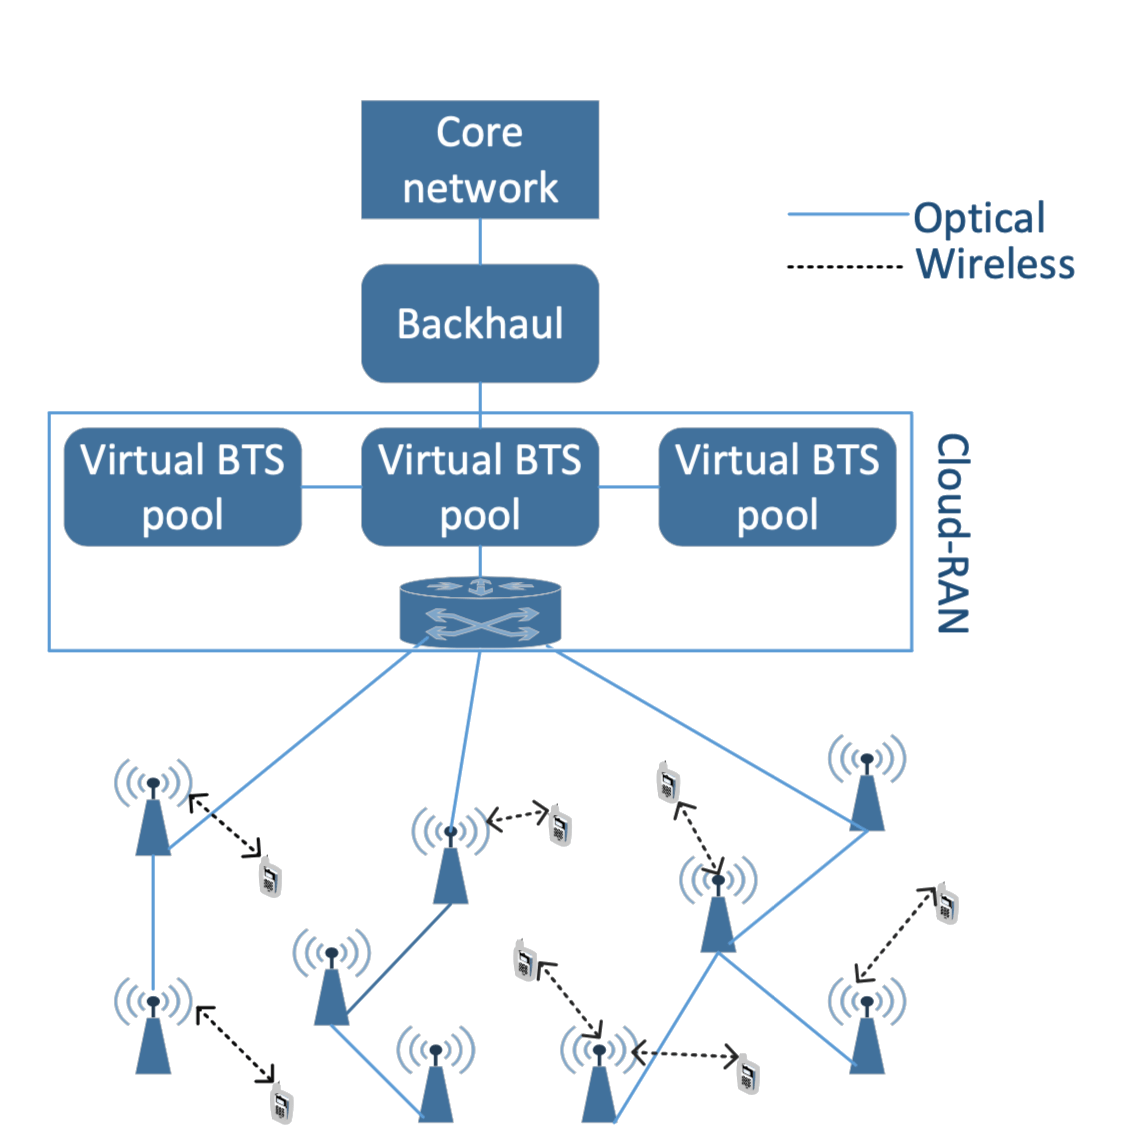
\includegraphics[width=0.5\textwidth]{./assets/cran.png}
  \caption{Cloud-RAN architecture in 5G networks.}
  \source{\cite{parvez2018survey}}
\end{figure}

An essential piece of the cellular network infrastructure is the \gls{RAN}. It provides wide-area wireless connectivity to mobile devices. The fundamental problem the \gls{RAN} solves is figuring out how best to use and manage limited spectrum to achieve this connectivity. In a dense wireless deployment with mobile nodes and limited spectrum, it becomes a difficult task to allocate radio resources, implement handovers, manage interference, and balance load between cells. As such, local geographical \gls{MNO} networks may be needed to effectively perform load balancing and interference management, as well as maximize throughput, global utility, or any other goal \cite{gudipati2013softran}.

Traditional radio access also has issues with power consumption and latency. This is problematic with \gls{5G} services, such as edge computing. To elaborate, the power spent on mobile users far from a cell may be significant. Regarding edge computing, this substantial transmit power may nullify all potential energy savings. One way to address this problem is by bringing the computational resources closer to the \gls{UE} \cite{barbarossa2014communicating} through increased cell deployments. In \gls{5G}, these increased deployments are closely-knit with the \gls{MEC} paradigm. In general, \glspl{MEC} are not a new way of thinking: similar approaches have been studied under different names, such as cyberforaging, \cite{sharifi2012survey}, grid technology \cite{foster2001anatomy}, computation offloading \cite{fernando2013mobile}, cloudlets \cite{satyanarayanan2009case}, and fog computing \cite{yi2015fog}. Conceptually \gls{MEC} differs from all these by positioning the computation resources to the mobile base stations \cite{blanco2017technology}.

To elaborate, \gls{MEC} could be defined as an architecture, which provides computing, storage, and networking resources within the \gls{RAN}. \gls{MEC} is part of the \gls{SDN} paradigm, and as such, is deployed on general-purpose hardware. \glspl{MEC} are defined to enable delay-sensitive, context-aware, high-bandwidth applications and insight, to be executed, and retrieved near the end-users. \glspl{MEC} alleviate backhaul usage and computation at the core network \cite{tran2017collaborative, blanco2017technology}, which in turn helps \glspl{MNO} to improve profit margins and reduce network costs \cite{saguna-intel2016}. Alleviated backhaul usage also reduces latency and improves the mobile users' experience \cite{tran2017collaborative}. \glspl{MEC} are owned and managed by the infrastructure provider, attached to the base stations \cite{blanco2017technology}. Studies suggest that resources of \glspl{MEC} could also be rented between \glspl{MNO} through network slicing \cite{samdanis2016network}.

\subsubsection{Hardware}

From a hardware perspective, the wireless access is being developed with three broad use case families in mind: \gls{eMBB}, \gls{mMTC}, and \gls{URLLC} \cite{tullberg2016metis}. Because spectral band often called "beachfront spectrum" has become nearly occupied, these access technologies rely on a relatively unused spectrum in the \gls{mmWave} range of 30–300 GHz, where wavelengths are 1–10 mm. The main reason that \gls{mmWave} spectrum lies idle is that, until recently, it had been deemed unsuitable for mobile communications. This is due to very short range transmission. However, semiconductors are maturing, their costs and power consumption falling and the other obstacles related to propagation are now considered increasingly surmountable \cite{andrews2014will}.

This, in turn, means the number of base station installations also need to increase. This is because increased frequencies decrease the distance and materials which the radio signal can travel \cite{parvez2018survey}. Other challenges related to hardware include that current cellular network services rely on \gls{DSP} units. \glspl{DSP} are proprietary devices that are purpose-built  \cite{sherry2012making, wang2011untold}. \glspl{DSP} have caused a problem for \glspl{MNO}: to make service additions or upgrades the whole \gls{DSP} has to be replaced \cite{li2015software}.

Additionally, integration with \gls{LTE} is necessary for quick and efficient deployment of \gls{5G}. In summary, \gls{5G} wireless access should be an evolution of \gls{LTE} complemented with architecture designs and radio technologies \cite{parvez2018survey}. As such, 5G-enabled devices having radios capable of \gls{LTE} communication is envisioned \cite{andrews2014will, larew2013air}. In such hybrid system, system information, control channel, and feedback are transmitted in the \gls{LTE} system, making the \gls{mmWave} spectrum available for data communication \cite{pi2011introduction}.

\subsubsection{Software}

Virtualization has been introduced to decouple software from hardware to address the aforementioned problems. Such installations are called \glspl{SDN} which make use of \glspl{NFV}. This essentially means that a \gls{RAN} can function on general-purpose hardware \cite{chowdhury2009network, chowdhury2010survey, schaffrath2009network}. What follows is that abstractions like container-orchestration systems, developed for decades \cite{burns2016borg} in software engineering, can be used to overcome challenges of \glspl{RAN} in \gls{5G}, such as dynamic resource allocation \cite{li2015software}.

\begin{figure}
  \centering
    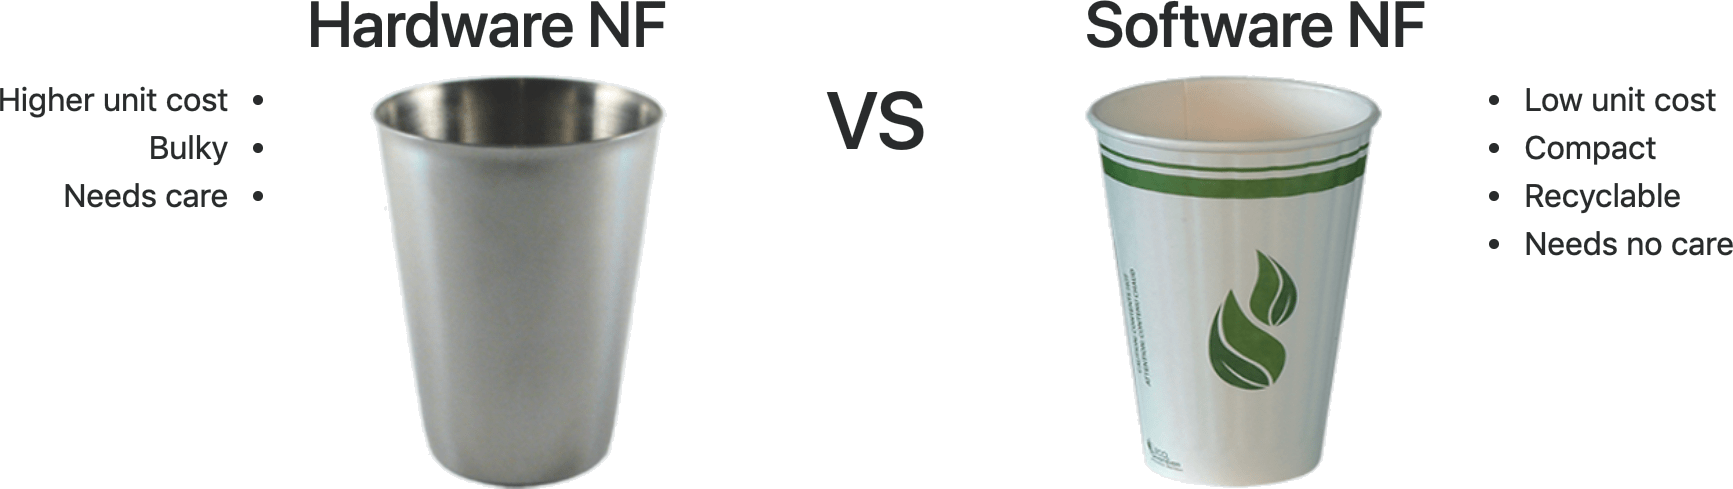
\includegraphics[width=\textwidth]{./assets/cups.png}
  \caption{Analogy which compares \gls{DSP}-based network functions with \gls{SDN}.}
  \source{Website of \cite{zaostrovnykh2017formally}.}
\end{figure}

In Release 15, \gls{3GPP} is defining \gls{5G} and its core network as the Next Generation Core. This essentially means that as a \gls{5G}-novelty, base stations and \glspl{EPC} are becoming intelligent edge computing resources. This can be considered to imply a change similar to which is envisioned with fog computing. As such, \gls{5G} also implies further decentralization of computer networks.

To elaborate, fog computing proposes a shift from cloud computing on datacenters towards a large number of geographically widespread edge nodes as part of a distributed and collaborating cloud. In \gls{5G} this is done via the \gls{MEC}-paradigm. Additionally, fog computing is defined to offer storage and to help offload traffic which would need to transverse the backbone. These are the same traits the \gls{MEC} is described to solve. However, the notion of fog computing nodes is wide: it defines that any equipment with processing power and storage, e.g., switches and routers, base stations, datacenters, and cloud platforms can be qualified as a fog node \cite{taleb2017multi}.

It could be considered that fog computing is the "holy grail" of distributed information networks in \gls{5G}. However, in comparison to the \gls{MEC}-paradigm, fog computing is envisioned to work in a trustless way. As such, the challenges are vast: at the edge of the network, user privacy and data security protection are the essential services that should be provided. Second is the ownership of the data collected from things at the edge. Just as what happened with mobile applications, the data of end user collected by things will be stored and analyzed at the service provider side \cite{shi2016edge}. However, with fog computing, the "service provider" might be your neighbor's refrigerator. As such, it can be considered a challenge whether leaving the data at the edge is any better for privacy than sending it to a data-silo. In other words, if nodes are interworking, how it can be programmatically ensured that the refrigerator protects user privacy?

In general, this problem domain could be defined as safe distributed trustless computing in decentralized networks. This implies more interest towards distributed network and application development. This field, in general, could be considered to have taken leaps of progression through projects like Ethereum, which allow applications on a decentralized, but singleton, compute resource. Ethereum calls this paradigm a transactional singleton machine with a shared-state \cite{wood2014ethereum}. This progress could be considered significant in terms of \gls{5G} and fog computing as well, because Ethereum is solving problems, such as execution model in a distributed state system. In \cite{wood2014ethereum} this is called a quasi-Turing complete machine. The paper proposes a parameter called "gas", which defines the amount of computation a node can request and execute using another node. While Ethereum only allows programs to be executed within its virtual machine, it could be envisioned that in the future more general-purpose programs could be executed, but which are still bound by similar intrinsic constraints.

Current cryptocurrency projects like Ethereum are not explicitly addressing this for the use of \gls{5G}, but the parallelism is evident. However, creating generic software out of the bounds of a virtual machine may be hard, as pointed out by \cite{whitman2011principles}: technical software failure, such as (1) buffer, integer and stack overflow, (2) string formatting problems, (3) race conditions, and (4) access to uninitialized or deallocated memory are all common problems with software, problems that result in software that is difficult or impossible to deploy in a secure fashion.

\subsection{Latency}

\begin{figure}
  \centering
    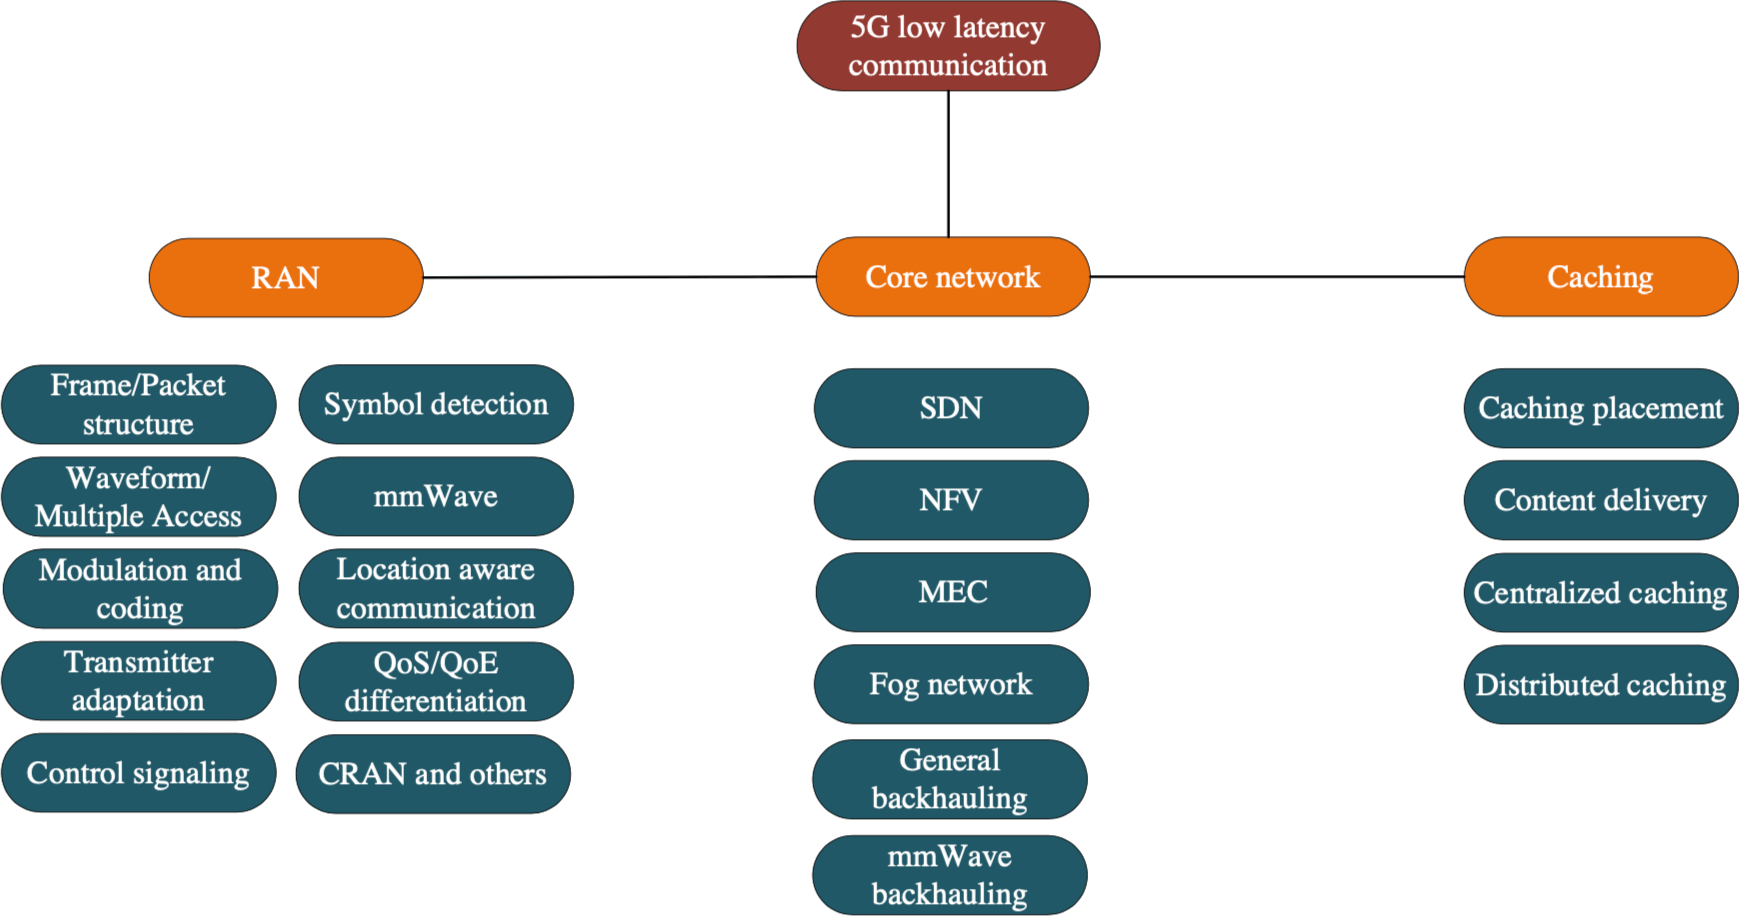
\includegraphics[width=\textwidth]{./assets/latency.png}
  \caption{Categories of different solutions for achieving low latency in 5G.}
  \source{\cite{parvez2018survey}}
  \label{fig:latencycat}
\end{figure}

\gls{E2E} latency can be considered to consist the sum of time to (1) send the program execution information from the mobile device to the cloud, (2) run the program at the remote side (cloud), and (3) the time to return results from the cloud back to the mobile unit \cite{barbarossa2014communicating}. Current \gls{LTE} \gls{E2E} latencies are on the order of about 10-15 milliseconds and are based on the one millisecond subframe time with necessary overheads for resource allocation and access. Although this latency is sufficient for most current services, anticipated \gls{5G} applications include two-way gaming, novel cloud-based technologies such as those that may be touchscreen activated, and \gls{VR} and \gls{AR}. As a result, \gls{5G} will need to support roundtrip latency an order of magnitude faster than \gls{LTE}. In addition to shrinking down the subframe structure, latency constraints may have significant implications on design choices at several layers of the protocol stack and the core network \cite{andrews2014will}.

In edge computing, we could further break down \gls{E2E} latency to be consisted of three different things, as measured in \cite{kamarainen2017measurement}: (1) device delay, (2) access delay, and (3) server delay. Determining adequate latency with \gls{E2E} edge computing can be considered to depend on the visual applications ran on the \glspl{UE}. For example, applications in \gls{AR} and \gls{VR} can be tied to a neurological process called \gls{VOR}. In \gls{VOR}, the brain coordinates eye and head movements to stabilize images on the retina. This is critical to synchronizing virtual and real objects to create a coherent immersion in \gls{AR}, for example. The \gls{VOR} process takes the brain seven milliseconds \cite{zheng2014minimizing}. \gls{VOR} is related to motion-to-photon latency, which \cite{anthes2016state} defines as the overall system lag. In VR, the maximum motion-to-photon latency should be 20 milliseconds. Frame rates lower than 20 milliseconds break the immersive experience and cause nausea \cite{anthes2016state}. This effectively means that the \gls{E2E} latency should be less than 20 milliseconds.

A further literature review reveals that little attention has been paid to practical \gls{E2E} reliability, latency, and energy consumption comprising both up and downlinks \cite{condoluci2016enabling}.  Studies like \cite{mezzavilla2018end} conclude that \gls{E2E} \gls{mmWave} technology also needs innovations across all layers of the communication protocol stack. Similar conclusions were found from existing protocol whitepapers, like that of \gls{UDT}. The \gls{UDT} whitepaper \cite{gu2007udt} concludes that the congestion control algorithm is the primary internal functionality to enable the use of high bandwidth effectively.

Considering the aforementioned, the subsections of this chapter go through each source of latency to better define the causes, and to evaluate possible bottlenecks and resolutions towards a zero latency \gls{5G} network.

\subsubsection{Device delay}

Combining the insight of \cite{kamarainen2017measurement, jacobs1997managing} we can consider following factors affecting the \gls{UE}: (1) input, (2) rendering, (3) display, (4) synchronization, and (5) frame-rate-induced delay. For this thesis, this could be further simplified into two categories determined by hardware components: (1) a gyroscope sensor and (2-4) the mobile graphics processing unit. We ignore frame-rate-induced delay because mobile displays achieving refresh rates of 144Hz and beyond are accessible by consumers today.

Prior art by \cite{lincoln2016motion} achieved rendering latency of 0.08 milliseconds per frame. This system used a local accelerated computing pipeline and could be considered, for this thesis, as the baseline rendering latency.

Study \cite{kamarainen2017measurement} used a remote rendering system with a Samsung S7 \gls{UE} as the client. In this case, the application is fully rendered in the \gls{WAN}, to which the \gls{UE} basically acts as a remote controller. This sort of remote computing using video can be considered an apt approach due to the interoperability of the medium. That is, as long as the content can be encoded as video, it does not matter whether the content consumed is \gls{AR}, \gls{VR} or video-games. The downside is that the \gls{UE} needs to decode and render video frames, which took the \gls{UE} about 25 milliseconds for a single h264 frame. Thus it can be concluded that with remote rendering systems looking to meet \gls{VOR} deadlines, the latency optimizations should primarily address the transport protocol, and the underlying video codec and its decoder implementation.

Research in \cite{suznjevic2016analysis} shows that Nvidia's remote rendering service uses \gls{RTP} over \gls{UDP}. As such, we could consider some recent developments to improve latency. For example, \cite{website:facebook-av1} concludes that recent video codecs such as \gls{AV1} achieve bit rate savings of around 40 to 50 percent over h264. The savings do not come free but are a trade-off of a much longer encoding process. Similarly, the transport protocol could be evaluated against novel approaches like \gls{QUIC}, which is designed to reduce latency \cite{langley2017quic} and have shown to improve \gls{QoS} under \gls{LTE} services when requesting web content \cite{qian2018achieving}. Initial studies on streaming content over \gls{QUIC} confirm increased video performance, albeit only when the packets do not need to travel over long physical distances \cite{bhat2017not}.

On the other hand, even if we suppose that we can copy the performance gains realized in \cite{website:facebook-av1}, we would still be left with an effective device delay of 12.5ms, considering the benchmarks of \cite{kamarainen2017measurement}. However, this latency does not yet include input delay, which according to \cite{kamarainen2017measurement} was found to be 12.2ms for a gyroscope. The sum of these two factors is already over 20ms. Because access and network delay are not yet considered, it can be deduced that further optimizations are required in consumer-grade \gls{UE} to provide immersive video-based experiences which make use of computation offloading in \glspl{RAN}.

\subsubsection{Access delay}

\begin{figure}
  \centering
    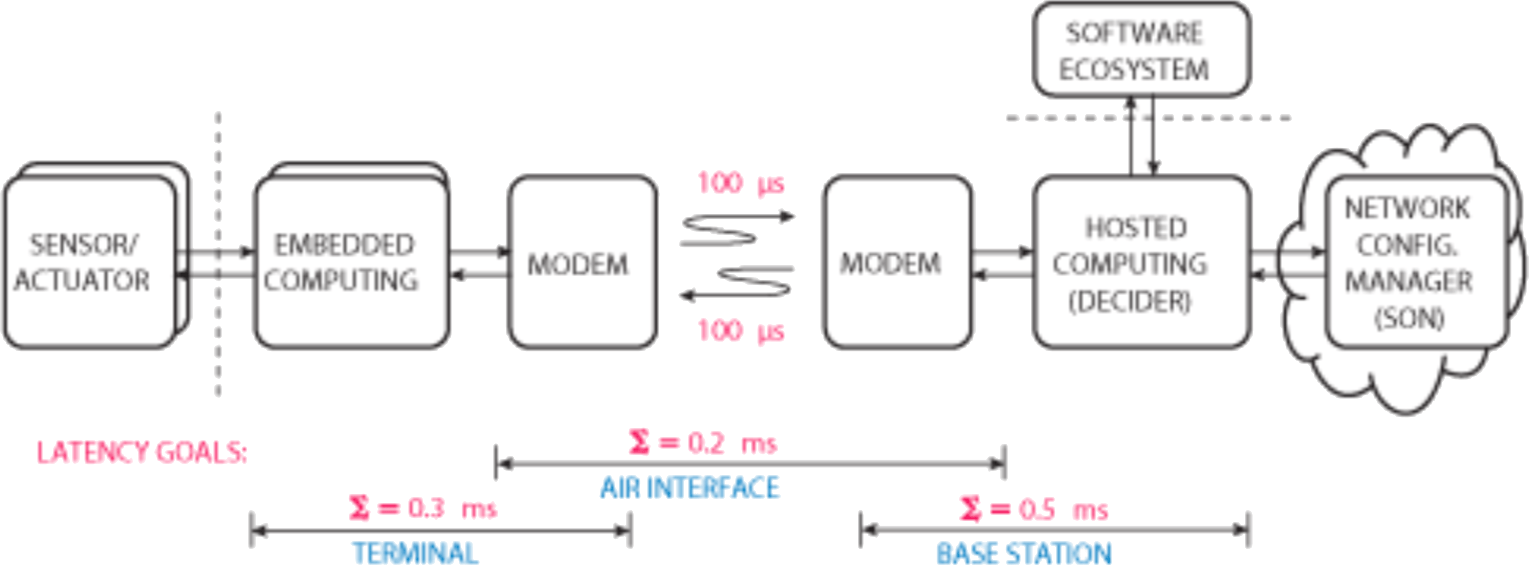
\includegraphics[width=\textwidth]{./assets/access.png}
  \caption{Breakdown of the 1 millisecond access delay in \gls{5G} \gls{UE}.}
  \source{\cite{fettweis20125g}}
  \label{fig:access}
\end{figure}

As depicted in figure \ref{fig:access}, access delay could be considered the sum of encoding, travel, and decoding of packets of the modems. In other words, access delay could be considered to be the actual wireless communication part in an \gls{E2E} setting. As such, latency optimizations in this interface could be considered very low-level in comparison to, e.g., rendering latency. Considering the categories defined in figure \ref{fig:latencycat}, the optimizations most accessible software-wise in this section could be considered to address frame and packet structure, and modulation and coding systems.

Due to its fundamental role in \gls{E2E} applications, it is difficult to achieve significant latency improvements without significant impact on the air interface. This is because of the latency relevant aspects such as frame structure, control signaling timing, and \gls{HARQ} form the critical building blocks of the air interface. For example, a round trip time requirement of 0.1 millisecond means that the \gls{TTI} length needs to be scaled down to 10-25~{\textmu s}. This cannot be achieved with the current \gls{LTE} \gls{OFDMA} numerology. As a solution to this problem, a scalable \gls{OFDMA} design is offered as a means to optimize the radio performance. In specific, reduction of \gls{CP}, the reference signal, and control signaling overhead are considered to provide a significant increase in throughput. It is worth noting that optimizations for efficiency and latency will be conflicting. Thus the system needs to provide adaptability to select configurations best supporting the specific services and applications used \cite{raaf2011vision}.

It is considered that a tunable \gls{OFDM} could be adapted in \gls{5G}. In particular, given the increasingly software-defined nature of radios, the \gls{FFT} block size, the subcarrier spacing, and the \gls{CP} length could change with the channel conditions: in scenarios with small delay spreads the subcarrier spacing could grow, and the \gls{FFT} size and the \gls{CP} could be shortened to lower (1) the latency, (2) the \gls{PAPR}, (3) the \gls{CP}'s power and bandwidth penalty, and (4) the computational complexity. In channels with longer delay spreads, that could revert to narrower subcarriers, longer \gls{FFT} blocks, and a longer \gls{CP} \cite{andrews2014will}.

It is also worth noting that, in comparison to device and network delay optimizations, optimizations in access delay may require spectrum licenses for empirical studies. For example, \cite{mezzavilla2018end, condoluci2016enabling, parvez2018survey} call for increased need for \gls{OTA} testing. It could be deduced to mean testing which includes real-world air interface interference in comparison to virtualized tests. Moreover, as mentioned earlier, optimizations in other layers could be considered to be always bounded by access delay. Thus, it could be considered essential to not forget about testing new findings in real-world scenarios.

Also, because of the bounding nature of the access delay, it could be considered that \gls{5G} \glspl{RAN} could even dynamically optimize its processing of access delay in the base stations. To elaborate, should there be a discovery mechanism for available hardware of the core network, given the depicted time of base station packet processing of 0.5 ms in figure \ref{fig:access}, it might make sense to use the optical connection to re-route the processing. In such a scenario, accelerated hardware residing in \glspl{MEC}, such as \glspl{FPGA}, could shorten not only the latency but also create more cost-effective base stations. To elaborate, if it could be assumed that base stations can schedule hardware from the \gls{MEC} and such hardware exists in the network, then one could, similarly to the vision of this thesis, remove computing capabilities from base station and instead rely on the \gls{MEC} to provide more cost-effective approaches for \glspl{RAN}. This could, in effect, used to reduce capital expenses of \glspl{MNO} to provide service by reducing the unit price of base stations.

\subsubsection{Network delay}

\begin{figure}
  \centering
    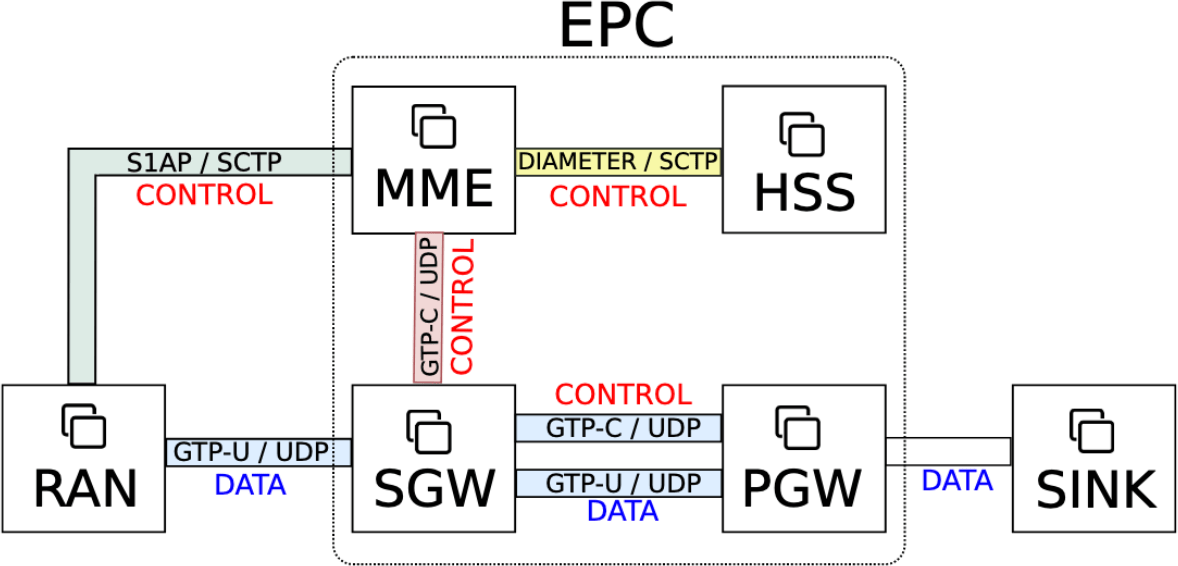
\includegraphics[width=\textwidth]{./assets/epc.png}
  \caption{\gls{NFV}-based \gls{LTE} \gls{EPC} implementation.}
  \source{\cite{jain2016comparison}}
  \label{fig:epc}
\end{figure}

Network delay is essentially the delay caused by the core network, i.e., the \gls{EPC} in the backhaul of the base stations. Figure \ref{fig:epc} demonstrates the essential parts of a \gls{LTE} \gls{EPC} and how these parts communicate technically between each other. Historically different parts of the \gls{EPC} have been run on custom-purpose \gls{DSP} hardware, hence the separation, but with \gls{SDN} the \gls{EPC} could technically operate under the same host computer.

In general, \glspl{RAN} are real-time applications, which require hard deadlines. This is to maintain protocol, frame, and subframe timings, and to perform transmission schemes such as beamforming, \gls{MIMO}, \gls{CoMP}, and Massive \gls{MIMO} \cite{nikaein2017towards}. \gls{DSP} systems can endorse these requirements through hardware design. However, this does not apply for software-based \glspl{RAN} which are powered by general-purpose processors. Instead, tuning the software environment to meet real-time processing is required. This essentially applies to the EPC as well. As so, \cite{mao2015minimizing} finds an optimized kernel essential for \glspl{RAN}. The study concludes that to overcome latency limitations of the Linux network stack (1) fine-tuned real-time kernel and (2) low-overhead virtualization hypervisor with kernel passthrough for \glspl{NIC} are needed.

\begin{figure}
  \centering
    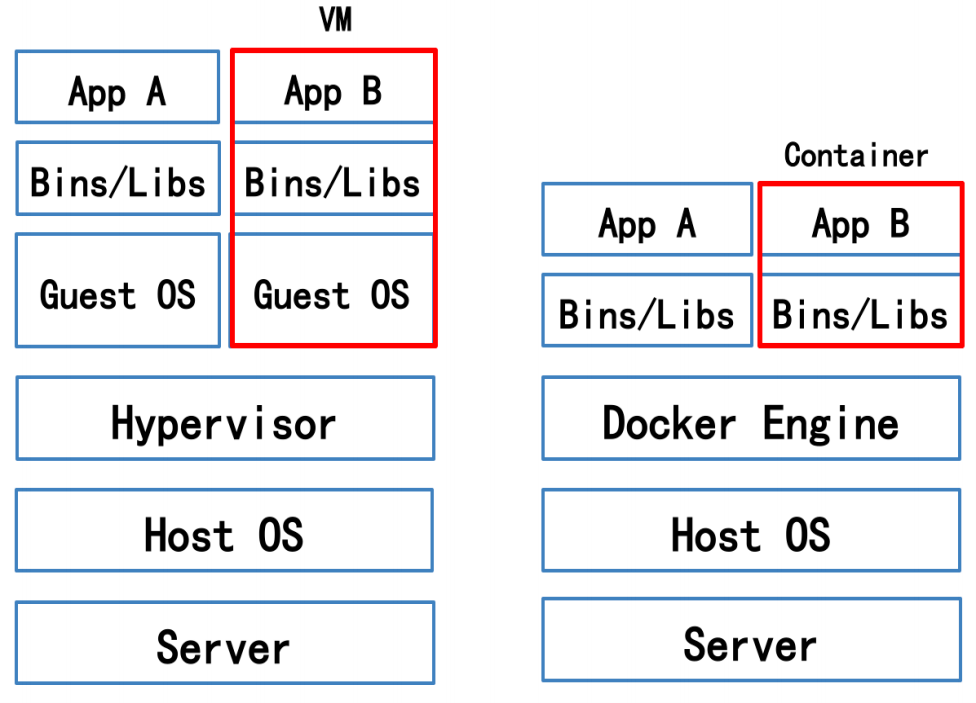
\includegraphics[width=0.5\textwidth]{./assets/docker.png}
  \caption{Architecture comparison of a virtual machine and a container}
  \source{\cite{zhang2018comparative}}
  \label{fig:docker}
\end{figure}

To elaborate, the \gls{5G} \gls{RAN} \gls{SDN}-paradigm defines the software to run in virtualized environments. However, this introduces processing overhead to applications, as demonstrated in figure \ref{fig:docker}: regardless of whether virtual machines or containers are used, there still exists abstraction layers which affect processing time. By introducing kernel passthrough technologies as suggested by \cite{mao2015minimizing}, one can essentially disregard the number of abstractions after the "Server" step and skip directly to the application "App" layer. These approaches reduce the processing so that the envisioned latency goals of \gls{5G} can be met through optimizations on the software-defined architecture \cite{mao2015minimizing}.

\newpage

\section{Contribution}
\label{ch:contribution}

\subsection{Review of OSS EPCs}

The University of Oulu has spectrum licenses to do \gls{OTA} testing. From the perspective of this thesis work, this means a \gls{LTE} network operated by the university is accessible at the campus to \gls{LTE} \glspl{UE}. The university owns the hardware of the \gls{RAN} and does not roam on an existing \gls{MNO}. This means that the university could be considered an independent \gls{MNO} and more specifically, a micro-operator \cite{ahokangas2016future}. The local infrastructure is detailed in more depth in thesis works, for example in \cite{arif2017msc}.

At the start of this thesis work, the infrastructure at Oulu University could have been considered proprietary by a software engineer. To elaborate, the base stations and the \gls{EPC} were using open and standardized protocols with abstractions offering software-based control. However, there was no kernel level access to these devices. In itself, this was not a limiting factor for latency studies in the \gls{UE} application layer. However, the \gls{EPC} of the infrastructure resided physically outside of the campus. This caused an \gls{E2E} latency of 50 milliseconds within devices in the same room. The \gls{EPC} was concluded to be the cause for the latency by intercepting the connection from a picocell to the \gls{EPC}. It was concluded that should a commercial micro-operator offer latency-optimized services, an \gls{EPC} residing in the \gls{WAN} would not likely mimic a production system. Thus to remove the network hop to the \gls{WAN}, it was deduced necessary to install an alternative \gls{EPC} to the campus' \gls{LAN}.

Additionally, the literature review on latency concluded that \glspl{RAN} require kernel optimizations \cite{mao2015minimizing}. Moreover, having a customizable \gls{RAN} was seen as useful in future research by faculty researchers. Considering these factors, an open-source alternative seemed useful. A brief literature review on open-source \glspl{EPC} was conducted. The following implementations of \glspl{EPC} were found and considered (listed in no particular order):
\begin{center}
    \begin{tabular}{ | l | l | p{10cm} |}
    \hline
    Project & Language & Anecdotal summary \\ \hline
    \href{https://github.com/acetcom/nextepc}{NextEPC} & C & Supports \gls{3GPP} Release 13 \\
    \hline
    \href{https://github.com/mitshell/corenet}{corenet} & Python & Minimal 3G and \gls{LTE} \gls{EPC} \\
    \hline
    \href{https://github.com/networkedsystemsIITB/NFV_LTE_EPC}{vEPC} & C++ & Developed with performance evaluation in mind \cite{jain2016comparison} \\
    \hline

    \href{https://gitlab.eurecom.fr/oai/openair-cn}{openair-cn} & C & "Probably the most complete open 4G project so far." \cite{website:spectrum-ieee} "[openair-cn] seems to be the most feature-complete implementation of all [open-source] solutions right now." \cite{website:srslte-mailinglist} \\
    \hline

    \href{https://github.com/srsLTE/srsLTE}{srsLTE} & C++ & "srsLTE have both the code elegance of openLTE and the completeness of [openair-cn]" \cite{website:cyberlog} \\
    \hline

    \href{http://openlte.sourceforge.net/}{openLTE} & C++ & "Ben Wojtowicz, almost single-handedly developed openLTE, an open-source \gls{LTE} software implementation, in his spare time." \cite{website:spectrum-ieee} \\
    \hline
    \end{tabular}
\end{center}

For its ease of installation, NextEPC was picked. The installation is specified in appendix \ref{ch:hardware}.

An open-source \gls{EPC} was found practical for micro-operator because of cost reductions. The same could apply to \gls{LTE} on an unregulated spectrum (\href{https://www.multefire.org/}{muLTEfire}) and rural deployments akin to \href{https://www.kuha.io/}{Nokia Kuha}. In general, open-source might also help to avoid security holes in \glspl{EPC}, which are known to exist \cite{shaik2015practical, rupprechtbreaking}. To elaborate, if the development would be open and accessible, more people could contribute towards a safe software by design. Whether these statements hold would need further research.

\subsection{OTA testing of latency-optimized OSS EPC}

Software-wise, \gls{LTE} and \gls{5G} are to coexist \cite{andrews2014will, larew2013air, pi2011introduction}. This means the software which translates a wireless signal to an Internet connection will be the same on \gls{LTE} and \gls{5G}. From this thesis' perspective, it means it is technically correct to use an \gls{LTE} \gls{UE} to measure the latency of a \gls{5G} \gls{RAN}. This is considered true because in general, \gls{5G} \gls{UE} is capable of offering better latency than \gls{LTE} \gls{UE} because of an improved air interface. What follows is any offloaded application, concerning \gls{E2E} latency, should perform better, or at least as well, on a \gls{5G} \gls{UE}.

Due to focus constraints of this thesis, further application development is left for future studies. Albeit, the following test results on latency are measured using commodity hardware specified in appendix \ref{ch:hardware}:

Running iperf3 and analyzing the traffic with Wireshark reveals that from 337'000 packets around 64'000 get a warning telling that \gls{TCP} frame is (suspected) to be out-of-order. In addition to this, around 2700 packets get a connection reset warning. This could be considered to imply performance bottlenecks in the \gls{EPC}'s software implementation or hardware.

Ping requests show that latency varies between 15 and 30ms when pinging from the \gls{EPC} host to the \gls{UE}. However, this ping varies on an either-or-basis, i.e., the ping tends to be either 15ms or 30ms, but not many results in between are seen.


\subsection{Discussion}

It can be deduced that \glspl{MEC} could also be used to form a new application distribution channel for software developers. Such applications could assume the low-latency guarantees and edge computing resources of the \gls{MEC}. A novel benefit is that the \glspl{MEC} is part of the network layer. Thus, such a platform would be an abstraction independent of the operating system of the \gls{UE}. For this reason, such a system could be considered a ubiquitous "App-Store layer" of \gls{5G}.

In agreement with \cite{saguna-intel2016}, it can be deduced that the \gls{MEC} architecture will become an essential component of \gls{5G}. However, this might not solely be for the end-user benefits. Instead, we can consider the \gls{MEC} also as an essential testing ground for \gls{E2E} research. To elaborate, \gls{MEC} can enable software engineers to take part in \gls{RAN} development through \gls{E2E} applications. This could be one natural vector of research interest towards technologies called upon in the literature review, regarding innovations in different parts of the \gls{RAN}.

\newpage

\section{Conclusions}

In the contribution chapter an \gls{LTE} \gls{UE}, a \gls{5G} \gls{MEC}, a micro-operator, an open-source \gls{EPC}, and software-based latency optimizations were combined. An empirical study proved that by utilizing \gls{MEC} an \gls{E2E} latency close to the practical limits of \gls{LTE} modems can be achieved. This suggests that micro-operators could, as of today, provide services unrealized by current \glspl{MNO}.

This thesis could be considered to pose grounds for further research to define the viability of the proposed infrastructure. For example, it could be practical to define the limits of \gls{QoS} which small \glspl{MNO} can offer in comparison to bigger ones. A continuation of latency research could also be considered. Either way, a more available spectrum policy would likely be helpful to realize the full capability of \gls{5G} radios to optimize the full \gls{E2E} latency. It can also be deduced that without liberal spectrum policies the findings of these approaches are likely hindered. This would, in effect, then affect the interests of the consumer and the broader market potential of \gls{5G}.

\newpage
\appendix
\newpage

\section{Relevant technical specification}
\label{ch:hardware}

Hardware-wise, the EPC consisted of Intel i3-6100T processor, Crucial 8GB DDR4 memory (CT2K4G4DFS824A), Asrock Z270 motherboard, and Samsung 250GB 850 EVO SSD.

The eNodeB used was Nokia FW2HHWC. The \gls{UE} used was a OnePlus A5010.

Software-wise, the EPC was running on Ubuntu 18.04 with kernel 4.16.15-rt7. The NextEPC environment was installed from the source. The git commit used was d004770.

\newpage
\bibliographystyle{apacite}
\bibliography{refs}

\end{document}

